\documentclass[landscape,a1paper,fontscale=0.424]{baposter}

\usepackage[vlined]{algorithm2e}
\usepackage{times}
\usepackage{calc}
\usepackage{url}
\usepackage{graphicx}
\usepackage{amsmath}
\usepackage{amssymb}
\usepackage{relsize}
\usepackage{multirow}

\usepackage{graphicx}
\usepackage{multicol}
\usepackage[T1]{fontenc}
\usepackage{ae}
\usepackage{enumitem}

\usepackage{booktabs}
\usepackage{colortbl}
\usepackage{xcolor}
%\usepackage{gensymb} % for \degree
\graphicspath{{figs/}}

\setlist[itemize]{leftmargin=*,nosep}
    \setlength{\columnsep}{0.7em}
    \setlength{\columnseprule}{0mm}

\setlist[enumerate]{leftmargin=2.5em,nosep}
    \setlength{\columnsep}{1.0em}
    \setlength{\columnseprule}{0mm}

\DeclareMathOperator*{\argmax}{arg\,max}
\DeclareMathOperator*{\argmin}{arg\,min}
% %%%%%%%%%%%%%%%%%%%%%%%%%%%%%%%%%%%%%%%%%%%%%%%%%%%%%%%%%%%%%%%%%%%%%%%%%%%%%%%%
% % Save space in lists. Use this after the opening of the list
% %%%%%%%%%%%%%%%%%%%%%%%%%%%%%%%%%%%%%%%%%%%%%%%%%%%%%%%%%%%%%%%%%%%%%%%%%%%%%%%%
% \newcommand{\compresslist}{%
% \setlength{\itemsep}{0pt}%
% \setlength{\itemsep}{0pt}%
% \setlength{\parskip}{0pt}%
% \setlength{\parsep}{0pt}%
% }
\renewcommand{\rmdefault}{ptm} % Arial
\renewcommand{\sfdefault}{ptm} % Arial

\newcommand{\vn}{\boldsymbol{n}}
\newcommand{\vl}{\boldsymbol{l}}
\newcommand{\vM}{\mathbf{M}}
\newcommand{\vN}{\mathbf{N}}
\newcommand{\vL}{\mathbf{L}}

\newcommand{\gradientcolor}[1]{\cellcolor{red!\the\numexpr80-#1*0.8\relax!yellow}}
%%%%%%%%%%%%%%%%%%%%%%%%%%%%%%%%%%%%%%%%%%%%%%%%%%%%%%%%%%%%%%%%%%%%%%%%%%%%%
%% Begin of Document
%%%%%%%%%%%%%%%%%%%%%%%%%%%%%%%%%%%%%%%%%%%%%%%%%%%%%%%%%%%%%%%%%%%%%%%%%%%%%
\begin{document}
%%%%%%%%%%%%%%%%%%%%%%%%%%%%%%%%%%%%%%%%%%%%%%%%%%%%%%%%%%%%%%%%%%%%%%%%%%%%%
%% Here starts the poster
%%---------------------------------------------------------------------------
%% Format it to your taste with the options
%%%%%%%%%%%%%%%%%%%%%%%%%%%%%%%%%%%%%%%%%%%%%%%%%%%%%%%%%%%%%%%%%%%%%%%%%%%%%
\begin{poster}{
        % Show grid to help with alignment
        grid=false,
        columns=5,
        % Column spacing
        colspacing=0.7em,
        % Color style
        headerColorOne=cyan!20!white!90!black, % changer les couleurs ?
        borderColor=cyan!30!white!90!black,    % changer les couleurs ?
        % Format of textbox
        textborder=faded,
        % Format of text header
        headerborder=open,
        headershape=roundedright,
        headershade=plain,
        background=none,
        bgColorOne=cyan!10!white,
        headerheight=0.12\textheight
    }
    % Eye Catcher
    {
        \includegraphics[width=0.1\linewidth]{logo/Sorbonne}
    }
    % Title
    {
        \sc\huge\bf ClimODE: Climate Forecasting With Physics-informed Neural ODEs
    }
    % Authors
    {
        \vspace{0.3em} Aymeric Delefosse$^{1}$ \enspace Mathis Koroglu$^{1}$ \enspace Charles Vin$^{1}$ \enspace $|$ \enspace Yogesh Verma$^{2}$ \enspace Markus Heinonen$^{2}$ \enspace Vikas Garg$^{2}$ \\[0.2em]
        \vspace{0.3em} \large $^{1}$Reviewers \enspace $^{2}$Original authors
    }
    % Other
    {
        \begin{tabular}{c}
            \raisebox{-1.0\height}{\includegraphics[width=0.15\linewidth]{logo/ICLR-logo}} \\
            % \raisebox{-0.7\height}{\includegraphics[width=0.16\linewidth]{images/QRCode_Link.pdf}}
        \end{tabular}
    }

    %%%%%%%%%%%%%%%%%%%%%%%%%%%%%%%%%%%%%%%%%%%%%%%%%%%%%%%%%%%%%%%%%%%%%%%%%%%%%%
    %%% Now define the boxes that make up the poster
    %%%---------------------------------------------------------------------------
    %%% Each box has a name and can be placed absolutely or relatively.
    %%% The only inconvenience is that you can only specify a relative position 
    %%% towards an already declared box. So if you have a box attached to the 
    %%% bottom, one to the top and a third one which should be inbetween, you 
    %%% have to specify the top and bottom boxes before you specify the middle 
    %%% box.
    %%%%%%%%%%%%%%%%%%%%%%%%%%%%%%%%%%%%%%%%%%%%%%%%%%%%%%%%%%%%%%%%%%%%%%%%%%%%%%

    %%%%%%%%%%%%%%%%%%%%%%%%%%%%%%%%%%%%%%%%%%%%%%%%%%%%%%%%%%%%%%%%%%%%%%%%%%%%%%
    \headerbox{\bf\color{blue} Problem Definition and Contribution}{name=contribution,column=0,row=0,span=2}{
        \textbf{\color{blue}Goal:} Enhancing climate forecasting by integrating physics-informed neural ordinary differential equations (ODEs) with uncertainty quantification.

        \textbf{\color{blue}Motivations:}
        \begin{itemize}
            \item Existing models neglect the underlying physics, lack of uncertainty quantification and are computationally intensive.
            \item Enhance efficiency and effectiveness in global and regional weather prediction tasks.
        \end{itemize}
    }

    \headerbox{\bf\color{blue} Problem Formulation}{name=formulation,column=0,below=contribution,span=2}{
        \textbf{\color{blue}Statistical Mechanics:} Weather can be described as a spatial movement of quantities over time, governed by the partial differential continuity equation:
        \vspace{-0.5em}
        \begin{equation*}
            \underbrace{\frac{du}{dt}}_{\text{time evolution }\dot u} + \underbrace{\overbrace{\mathbf{v} \cdot \nabla u}^{\text{transport}} + \overbrace{u \nabla \cdot \mathbf{v}}^{\text{compression}}}_{\text{advection}} = \underbrace{s}_{\text{sources}},
            \vspace{-0.5em}
        \end{equation*}
        where $u(x, t)$ is a quantity evolving over space $\mathbf{x}$ and time $t$ driven by a flow's velocity $\mathbf{v}(\mathbf{x}, t)$.

        \textbf{\color{blue}Main Idea:} We solve the continuity equation over entire Earth as a system of neural ODEs. % We learn the flow $\mathbf{v}$ as a neural network that uses both global attention and local convolutions and address source variations via a probabilistic emission model that quantifies prediction uncertainties.
    }

    \headerbox{\bf\color{blue} Method}{name=abstract,column=0,below=formulation,span=2}{
        \textbf{\color{blue}Network Architecture:}
        Spatiotemporal embedding $\psi$ encodes time and location information to capture cyclical patterns of day and season.
        \vspace{-1em}
        \begin{center}
            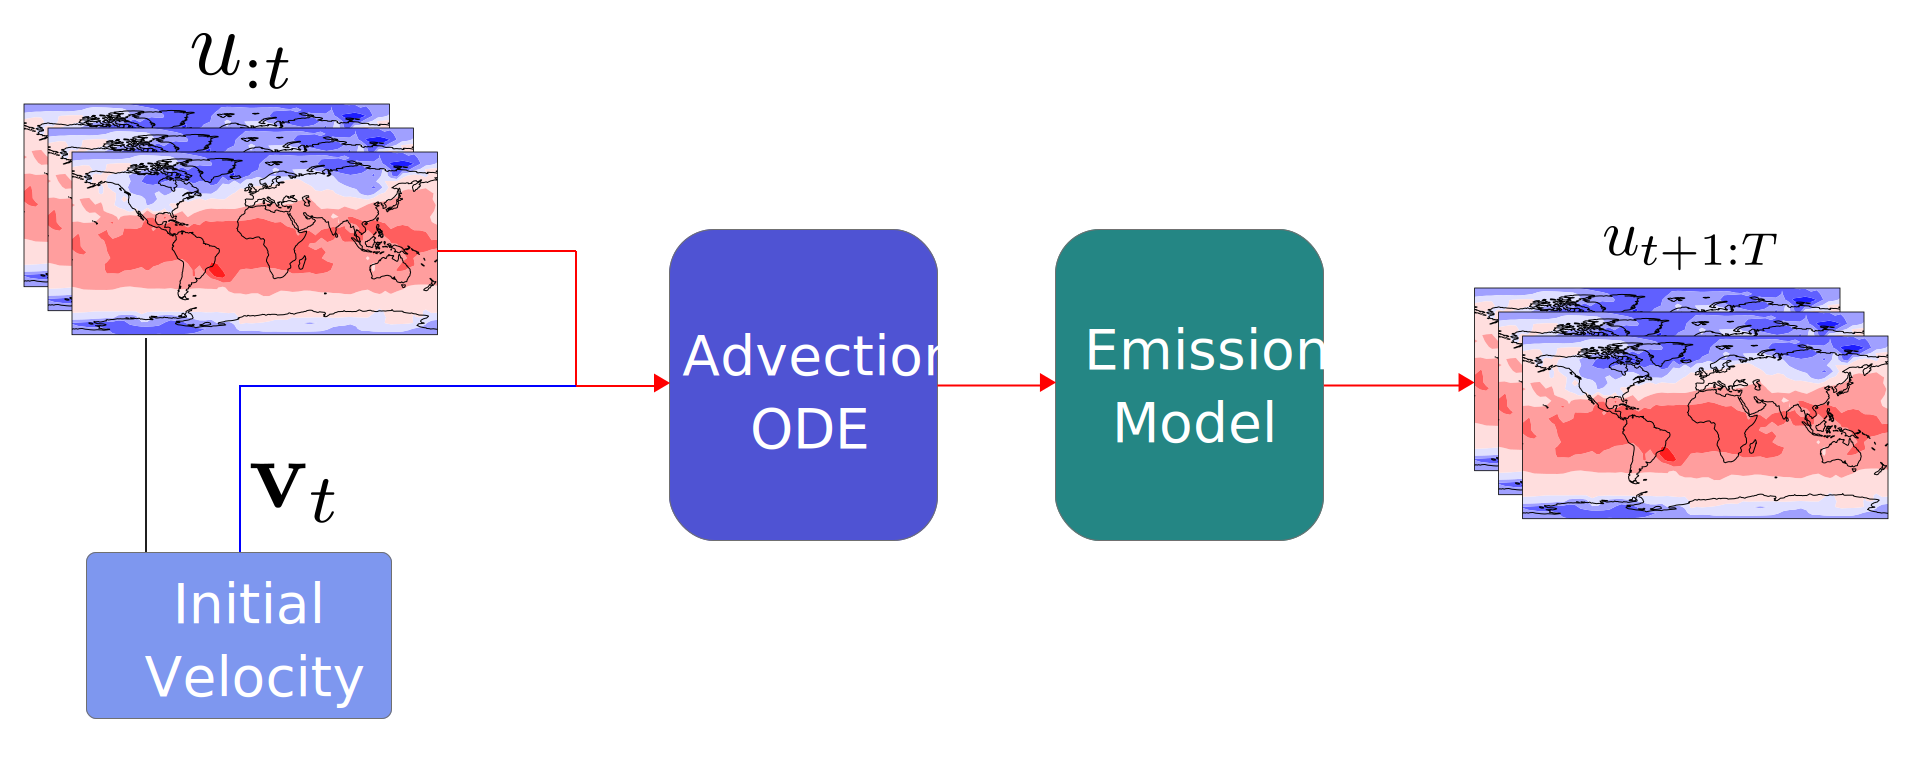
\includegraphics[width=0.48\textwidth]{ClimODE.pdf}
            \includegraphics[width=0.48\textwidth]{AdvectionODE.pdf}\\
            \makebox[0.48\textwidth]{\small (a) ClimODE}
            \makebox[0.48\textwidth]{\small (b) {Advection ODE}}
            \vspace{-0.5em}
        \end{center}

        % \begin{center}
        %     % \hfill
        %     % \includegraphics[width=0.5\textwidth]{AdvectionODE.pdf}
        %     % \includegraphics[width=\textwidth]{pipeline.pdf}
        % \end{center}
        % \vspace{-0.5em}
        %
        \textbf{\color{blue}Initial Velocity Inference:}
        \vspace{-0.5em}
        \begin{equation*}
            \hat{\mathbf{v}}_{k}(t) = \argmin_{\hat{\mathbf{v}}_{k}(t)} \left\{ \big\Vert \tilde{\dot{u}}_k(t) + \mathbf{v}_{k}(t) \cdot \tilde{\nabla}u_k(t) + u_k(t) \tilde{\nabla} \cdot \mathbf{v}_k(x,t) \big\Vert_2^2 + \alpha \big\Vert \mathbf{v}_k(t) \big\Vert \right\}
        \end{equation*}
        %
        \textbf{\color{blue}Advection ODE:} Modeling the dynamic evolution of quantities at specific locations by transforming second-order PDEs into first-order ODEs:
        \vspace{-0.5em}
        \begin{equation*}
            \begin{bmatrix}\mathbf{u}(t) \\ \mathbf{v}(t)\end{bmatrix}
            % = \begin{bmatrix}\mathbf{u}(t_0) \\ \mathbf{v}(t_0)\end{bmatrix} + \int_{t_0}^{t} \begin{bmatrix}\dot{\mathbf{u}}(\tau) \\ \dot{\mathbf{v}}(\tau) \end{bmatrix}  \,d\tau 
            = \begin{bmatrix} \{u_k(t_0)\}_k \\ \{ \mathbf{v_k}(t_0) \}_k \end{bmatrix} + \int_{t_0}^{t} \begin{bmatrix} \{  - \nabla \cdot \left( u_k(\tau)  \mathbf{v}_k(\tau) \right) \}_k \\ \{ f_{\theta}(\mathbf{u}(\tau), \nabla \mathbf{u}(\tau), \mathbf{\tau}(t), \psi)_k  \}_k \end{bmatrix} \,d\tau
        \end{equation*}
        %
        \textbf{\color{blue}Flow Velocity:} Modeling local and global effects using a hybrid network:
        \vspace{-0.5em}
        \begin{equation*}
            \dot{\mathbf{v}}_k(x,t) = f_{\text{conv}} \left( \mathbf{u}(t), \nabla \mathbf{u}(t), \mathbf{v}(t), \psi \right) + \gamma f_{\text{att}} \left( \mathbf{u}(t), \nabla \mathbf{u}(t), \mathbf{v}(t), \psi \right) % f_{\theta}(\mathbf{u}(t), \nabla \mathbf{u}(t), \mathbf{v}(t), \psi) 
        \end{equation*}
        %
        \textbf{\color{blue}Emission Model:} Accounting for uncertainty and value changes in climate estimates:
        \vspace{-0.5em}
        \begin{equation*}
            u_{k}^{\mathrm{obs}}({\bf x},t)\sim{\cal N}\left(u_{k}({\bf x},t)+\mu_{k}({\bf x},t),\sigma_{k}^{2}({\bf x},t)\right), \quad \mu_{k}({\bf x},t),\sigma_{k}({\bf x},t)=g_{k}\left({\bf u}({\bf x},t),\psi\right)
        \end{equation*}
        \vspace{-0.5em}
        %
        \textbf{\color{blue}Loss Function:} Gaussian negative log-likelihood: %of the observations $\mathbf{y}_i \in \mathbb{R}^{K \times H \times W}$ at times $t_i$ :
        \vspace{-0.5em}
        \begin{equation*}
            \mathcal{L}_{\theta} = - \frac{1}{NKHW} \sum_{i=1}^{N} \left( \log \mathcal{N}\left(\mathbf{y}_{i}|\mathbf{u}(t_{i}) + \boldsymbol{\mu}(t_{i}), \text{diag}\ \boldsymbol{\sigma}^{2}(t_{i})\right) + \log \mathcal{N}_{+}\left(\boldsymbol{\sigma}(t_{i})|\boldsymbol{0},\lambda_{\sigma}^{2}I\right) \right)
        \end{equation*}
    }
    %
    \headerbox{\bf\color{blue} Experiments \& Results}{name=results,column=2,row=0,span=3}{
        \begin{minipage}[t]{0.50\textwidth}
            \textbf{\color{blue}Effect of Emission Model:}
            \vspace{-0.5em}
            \begin{center}
                \includegraphics[width=0.4\textwidth]{bias_effect.png}\\
                \makebox[0.48\textwidth]{\small (a) Bias $\mu(\mathbf{x}, t)$}
                \makebox[0.48\textwidth]{\small (b) Std $\sigma(\mathbf{x}, t)$}
                \includegraphics[width=0.48\textwidth]{mu.pdf}
                \includegraphics[width=0.48\textwidth]{std.pdf}
            \end{center}

            \textbf{\color{blue}Quantitative Results and Comparison on ERA5:}
            \vspace{-0.5em}
            \begin{center}
                % \includegraphics[width=\textwidth]{acc.pdf}
                % \includegraphics[width=\textwidth]{rmse.pdf}
                \includegraphics[width=\textwidth]{acc_rmse.pdf}
            \end{center}
        \end{minipage}\hfill
        \begin{minipage}[t]{0.50\textwidth}
            \textbf{\color{blue}Effect of Individual Components:}
            \vspace{-0.5em}
            \begin{center}
                \includegraphics[width=\textwidth]{ablation.png}
            \end{center}

            \textbf{\color{blue}Quantifying Climate Interdependencies:}
            \vspace{-0.5em}
            \begin{center}
                \includegraphics[width=0.9\textwidth]{pairwise.pdf}
            \end{center}
        \end{minipage}

        \begin{minipage}[t]{0.48\textwidth}
            \vspace{0.5em}
            \textbf{\color{blue}Effect of ODE Solver (per batch, on a single A100):}\\[0.2em]
            \begin{tabular}{lcccccc}
                \hline
                Solver & \multicolumn{2}{c}{Euler} & \multicolumn{2}{c}{RK4} & \multicolumn{2}{c}{Implicit Adams} \\
                Adjoints & w & w/o & w & w/o & w & w/o \\
                \hline
                Time (s) & {\cellcolor[HTML]{FEDDBC}} \color[HTML]{000000} 0.27 & {\cellcolor[HTML]{FFF5EB}} \color[HTML]{000000} 0.18 & {\cellcolor[HTML]{FDBF86}} \color[HTML]{000000} 0.34 & {\cellcolor[HTML]{FDCFA0}} \color[HTML]{000000} 0.31 & {\cellcolor[HTML]{7F2704}} \color[HTML]{F1F1F1} 0.69 & {\cellcolor[HTML]{FA8532}} \color[HTML]{F1F1F1} 0.45 \\
                VRAM (Gb) & {\cellcolor[HTML]{FFF5EB}} \color[HTML]{000000} 10.2 & {\cellcolor[HTML]{FDC997}} \color[HTML]{000000} 15.7 & {\cellcolor[HTML]{FEECD9}} \color[HTML]{000000} 11.8 & {\cellcolor[HTML]{FDAD69}} \color[HTML]{000000} 17.8 & {\cellcolor[HTML]{FEDDBC}} \color[HTML]{000000} 13.7 & {\cellcolor[HTML]{7F2704}} \color[HTML]{F1F1F1} 30.1 \\
                \hline
            \end{tabular}
        \end{minipage}\hfill
        \begin{minipage}[t]{0.5\textwidth}
            \vspace{0.5em}
            \textbf{\color{blue}~~Validity of Mass Conservation:}
            \vspace{-0.5em}
            \begin{center}
                \includegraphics[width=\textwidth]{mass_conservation.pdf}
            \end{center}
        \end{minipage}
    }
    %
    \headerbox{\bf\color{blue} Critics}{name=critics,column=2,below=results,span=3}{
        \begin{minipage}[t]{0.48\textwidth}
            \textbf{\color{blue}Paper:}
            \begin{itemize}
                \item Lacks comparison to other models, such as FourCastNet, FuXi or Pangu-Weather (WeatherBench2)
                \item Is the comparison against ClimaX fair?
                \item Benchmark only up to 36 hours while state-of-the-art methods reported results for up to 10 days ahead
                \item Why choose ResNet over U-Net to model Gaussian prior for capturing both aleatoric and epistemic variance in the Emission Model?
            \end{itemize}
        \end{minipage}\hfill\begin{minipage}[t]{0.48\textwidth}
            \textbf{\color{blue}Implementation (original code):}
            \begin{itemize}
                \item Concerns about data leakage
                \item Absence of shuffling - impact?
                \item Unclear handling of residual architecture and dropout
                \item Code quality critique: Concerning coding standards
                \item Using Euler scheme to solve the ODE is known to be unstable but is a good compromise in terms of accuracy and efficiency
            \end{itemize}
        \end{minipage}
    }
    %
\end{poster}
\end{document}
